\section{Progressive JPEG Manipulation (ms)}
\label{sec:implementation_progressive_jpeg}

\subsection{Introduction}

For information on the reasoning behind implementing 
progressive JPEG manipulation, please see 
the JPEG manipulation section in the 
Approaches considered section. (see section \ref{sec:jpegmanipulation}).

The progressive JPEG manipulation algorithm was planned to be
done in this way:

\begin{enumerate}
	\item Extract the JPEG information from the JPEG headers 
		using the AVR microcontroller.
	\item Send the necessary image data for a low detail
	         version of the picture (includes both header information
		and entropy-encoded image data) to the ground station.
	\item Decode the image data received at the ground station.
	\item Progressively display the image on the ground station.
	\item Repeat stages 2 through 4, increasing the detail resolution 
		each time until all the image data has been sent for a perfect 
		representation of the photograph.
\end{enumerate}

The JPEG headers contain all the information needed to
recreate the compression of the concerned image. This includes
the Huffman table codes and quantization table coefficients,
which give precise information on how the image has been encoded.
Because these values are dependent on the properties of the image
(colour differences of adjacent cells, frequency of colours, etc.), it
is not possible to apply an algorithm to display JPEG images without
taking into account these properties of the image.

In order to extract the necessary JPEG information from
the headers, a JPEG information extractor would be
programmed in C and implemented on the AVR microcontroller.
Software on the ground station would then 
receive the incomplete image data and
progressively display an image to the user using the Huffman
and quantization tables obtained from the AVR.

The AVR based JPEG information extractor has undergone
three major revisions. A functional prototype was first
implemented in C\# due to familiarity with the coding language.
When the C\# prototype started reacting properly to 
jpeg testing images, the code was translated to C to be
implemented with the AVR. In order to be able to test
the extractor before implementing it onto the AVR, an 
executable C version of the extractor would be designed
to be able to read JPEG images and print the extracted
information on a console.

At the end of the project development period, only the 
extractor was successfully implemented. The C executable 
version of the extractor has been fully tested against 
a range of test images. A form of image displaying 
software has also been constructed which uses the 
Huffman table information obtained from the extractor, 
but a progressively higher resolution display of 
the image was not able to be fully implemented.

\subsection{AVR Header Search (commandCheck)}

The JPEG extractor will be able to obtain the 
number of packets the camera is sending directly from the camera.
After receiving the size of the JPEG file (in bytes), 
the JPEG Information Extractor would read the bytes of the JPEG stored in the SD card. 
Because the information will not all be available instantly, 
the extractor uses a class to read the next byte in the input stream, one at a time. 
This C class \textbf{read\_byte()} (see appendix \ref{}) is how the JPEG extractor 
gains access to the JPEG input stream. 

As the extractor reads in the bytes from the input stream, it checks to see if the byte indicates the start of a header (0xff). 
If this is the case, the next byte identifying the header is read and the \textbf{JPEGMethod()} class  (see appendix \ref{}) is 
called which uses a switch command to determine the actions to take. 
If not, the data is discarded and the extractor continues 
to read the next byte from the input stream. 

\subsection{AVR Header Data Extraction (JPEGMethod)}

The JPEG information extraction class does not need all the possible information that can be extracted from a JPEG image. 
The few image headers containing important information store the important information from the input stream into 
variables which will be sent to the custom encoding algorithm. 

If the header is not recognized by this class, 
it is assumed to not have any important information and is ignored; 
the code continues to scan through the input stream for the next header byte. 
Below is a list of headers the extractor obtains important information from 
and an explanation of the intended purpose of the values it extracts. 
Refer to appendix \ref{chap:jpeg-segment-contents} for information on the full contents of each
of the segments.

\subsubsection{SOF0: Start Of Frame (0xc0)}

The extractor mostly obtains general information from the SOF0 segment. 
It saves the height and width of the image for the ground station
software to prepare the progressively scanned image's dimensions
and keeps the data precision as a basic means of error checking. 
If the data precision is not 8, indicating a byte, then the image will not
be able to be read by the ground station.

The number of components helps indicate the colour space which will
be used. Ideally, the image will use the YCbCr colour space. Currently,
there is no functionality for Y, I, and Q components  which is not
used by UK-based cameras. Grey-scale images have yet to be
tested with the extractor.

The sampling factor information from this section will indicate
the chroma subsampling pattern used (either 4:2:2 or 4:2:0)
and influence the shape of the chrominance pixel structures
created during the treatment of the SOS segment. The 
sampling factor information will also define the dimensions of the
MCU (8x8 or 16x16).

Below is a screen shot taken from the executable version of
the JPEG information extractor from a standard JPEG image.
All screenshots were taken from the console of the Eclipse
development environment.

\begin{figure}[!hbtp]
\begin{center}
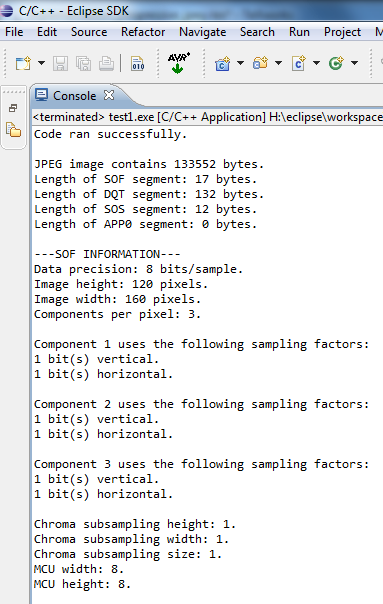
\includegraphics[scale=1]{figures/SOFOutput.png} 
\end{center}
\caption{SOF information obtained from the executable}
\end{figure}

\newpage
\subsubsection{DHT: Define Huffman Table(s) (0xc4)}

Obtaining the Huffman table information is vital for the
progressive scanning of the image to function properly.
Due to the fact that JPEG images are Huffman-encoded,
it is necessary to obtain the Huffman table information
used to encode them in order to decode the image
data properly into a visible format.

Each DHT segment may contains multiple Huffman tables.
Usually, one DHT segment would contain a pair of Huffman 
tables, one for DC and one for AC, to be used for image
decoding. Additionally, testing has revealed that 
multiple DHT segments may exist in a single JPEG file.

The extractor creates a unique Huffman table structure to
store all the information from the DHT segment. This information
is stored within a linked list of these Huffman table structures.

In order to choose the correct Huffman table among the many
tables which are used, the JPEG file issues an identification number
to each Huffman table which is shared only by its DC/AC counterpart.
The Huffman table structure keeps this information as well as the
DC or AC nature of each Huffman table so that the ground station
software can easily find the appropriate Huffman table to use to
decode a pixel component.

After storing the classification details of the Huffman table,
the extractor analyses the number of symbols for each
of the code lengths 1\ldots16. It then creates arrays
of appropriate sizes to store all symbols contained in 
the Huffman table. The organization of this data allows
a full Huffman table to be reconstructed using one
Huffman table struct, as shown below:

\begin{figure}[!hbtp]
\begin{center}
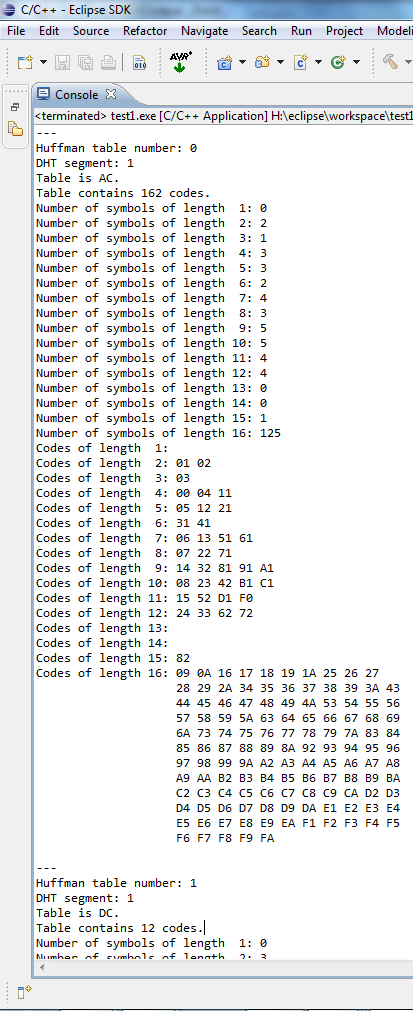
\includegraphics[scale=0.5]{figures/DHTOutput.png} 
\end{center}
\caption{DHT information obtained from the executable}
\end{figure}

%% Comment out until code is fixed
%%\subsubsection{DQT: Define Quantization Table(s) (0xdb)}
%%
\subsubsection{SOS: Start Of Scan (0xda)}

The SOS segment is the final header containing JPEG
compression information before the entropy-encoded
image data is read in. It specifies the AC and DC Huffman tables
which must be associated with each component in the scan.
The JPEG information extractor uses this information to be
able to assign each entropy encoded image byte with
the Huffman tables used to encode it. This way, the 
ground station image decompression algorithm can 
easily associate each image byte with an operation to
reverse the Huffman table modification in order to display
the original image.

\subsection{Image Data Treatment}

As explained in section (\ref{sec:entropycrho}), the entropy-encoded
image data would be stored in chrominance pixel structures. This structure
stores information for all the luma values within the chrominance pixel, 
as well as both chrominance values associated with it. Specifically, it contains:
\begin{itemize}
	\item An ID number to keep track of the image bytes.
	\item The AC Huffman table ID number of each of the components.
	\item The DC Huffman table ID number of each of the components.
	\item The value of the component.
\end{itemize}
If the ground station software needs to determine what 
component the byte value corresponds to, it will need to identify either 
the order of appearance of the components (ID number) or the 
Huffman table information of the components.
If we consider \emph{n} to be the number of image pixels in a chrominance pixel, then 
we associate the first $n - 2$ bytes with the Y (luma) Huffman tables, the $n - 1$ byte with the Cb Huffman tables, and 
the $n^{th}$ byte with the Cr Huffman Table. 
This information continues to be read by the extractor 
until the EOI header is found, or until there are no more bytes coming in from the input stream.


